% Chapterd Dodatek A
\chapter{Mapowanie portów procesora BCM2836} % Chapter title

\label{ch:BCM2836} % For referencing the chapter elsewhere, use \autoref{ch:name} 

Mapowanie portów procesora BCM2836 
Wyprowadzenia portów GPIO na płycie są identyczne w przypadku płyt Raspberry Pi, Raspberry Pi rev. B i Raspberry Pi 2 rev. B – jest to 40 złączy typu goldpin. Jednak wraz ze zmianą jednostek SoC w poszczególnych wersjach płyt zmianie uległy też rozkład i funkcje odpowiednich pinów.
Biblioteka wiringPi dostarcza wygodny interfejs obsługi portów GPIO układów z rodziny Raspberry Pi, dzięki któremu programista nie musi sprawdzać tych portów, zapewniając przenośność kodu między różnymi wersjami urządzeń.
 Autor biblioteki proponuje własny schemat numeracji pinów rozpoczynający się od GPIO0 do GPIO7 na głównym złączu P1. Oprócz tego dostępne są też porty specjalnego przeznaczenia jak np. złącza SDA i SCL interfejsu I2C.

\begin{figure}[bth]
\centering
{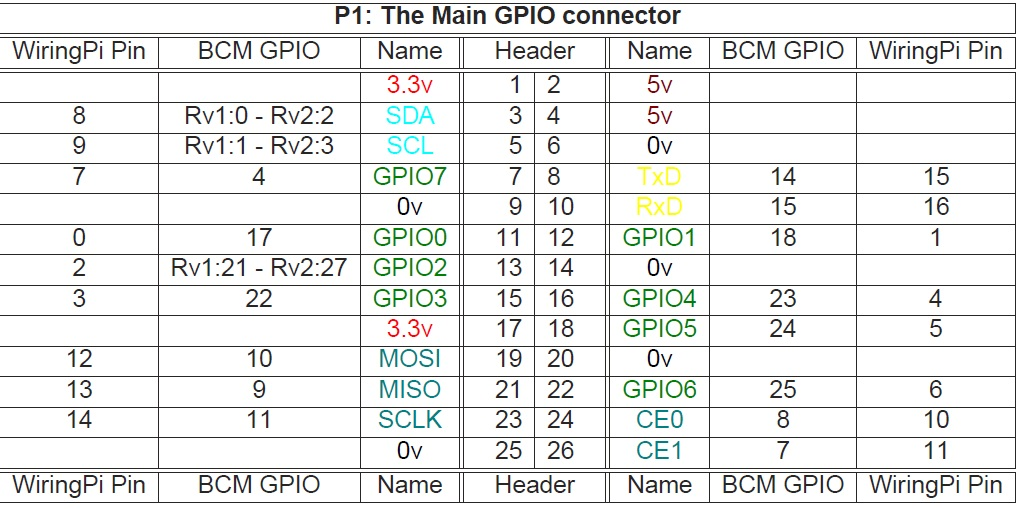
\includegraphics[width=1\linewidth]{sch/pinMap}}
\caption[Mapowanie portów GPIO biblioteki wiringPi.]{Mapowanie portów GPIO biblioteki wiringPi.}
\label{fig:detObj}
\end{figure} 